\subsection{ソフトウェアエンジニアリング運用ツール}

運用ツールは、人的資源を効率よく使い、品質と応答速度を高めるために重要である。適切に実装された自動化は、手作業より速く、容易で、信頼性が高い。DevOpsでは、開発、保守、運用の資源と手順を結びつけ、継続的インテグレーション、継続的デリバリー、継続的テスト、継続的デプロイを支援する。

継続的デリバリーは、新しいシステムやソフトウェアを頻繁に試験環境や事前本番環境へ届ける実践である。継続的テストは、ソフトウェアライフサイクルの各段階で品質を評価する実践である。継続的デプロイは、自動検証を通過した変更を本番へ自動配備するプロセスである。

\subsubsection{コンテナと仮想化}

コンテナと仮想化は、アプリケーションの拡張性を高め、複数のサーバやクラウド提供者にまたがる配備を標準化するために使われる。コンテナは、アプリケーションと実行に必要な依存関係をまとめ、環境差分を減らす。仮想化は、物理サーバ上に複数の仮想サーバを作る。

運用担当技術者は、プロジェクトの規模、複雑さ、柔軟性、セキュリティ、監視要求に基づいてツールを選ぶ。コンテナ管理ツール、すなわちオーケストレータは、多数のコンテナの配備、再起動、スケーリング、ネットワーク、監視を支援する。

\subsubsection{配備}

配備ツールは、さまざまな環境へのソフトウェア配備を管理する。配備記述ファイル、設定ファイル、環境変数、シークレット管理、コンテナイメージ、クラウド資源、データベース変更などを扱う。

実務では、一つのツールだけで全体をまかなうことは少ない。ビルド、パッケージ、インフラ作成、設定管理、データベース移行、監視、アラート、ロールバックなど、複数のツールを組み合わせて配備パイプラインを構築する。

\subsubsection{自動テスト}

開発者へ速く継続的なフィードバックを提供するため、テストはソフトウェア提供プロセス全体で可能な限り自動化されるべきである。単体試験、統合試験、システム試験、利用者受け入れ試験を含む試験戦略を定義し、それぞれを支援するツールを選ぶ。

自動テストは、単に欠陥を検出するだけではない。変更が安全に本番へ進めるかを判断する門番である。自動テストが不十分だと、配備を速くするほど障害を速く広げてしまう。

\subsubsection{監視とテレメトリ}

監視とテレメトリは、運用の中核である。監視は、サービスが正常かどうかを観察する活動である。テレメトリは、システムからデータを収集して分析に使う仕組みである。

監視では、アプリケーション層のログ、オペレーティングシステム層の実行トレース、サーバ層のCPU使用量やメモリ使用量などを収集する。収集されたデータには、統計分析や機械学習を使って意味を抽出できる。最終的には、ダッシュボードにより、開発者、運用者、製品責任者、経営層など、異なる利害関係者に必要な情報を見せる。

\begin{figure}[htbp]
\centering
\IfFileExists{assets/generated_figures/ch06/fig-ch06-12.png}{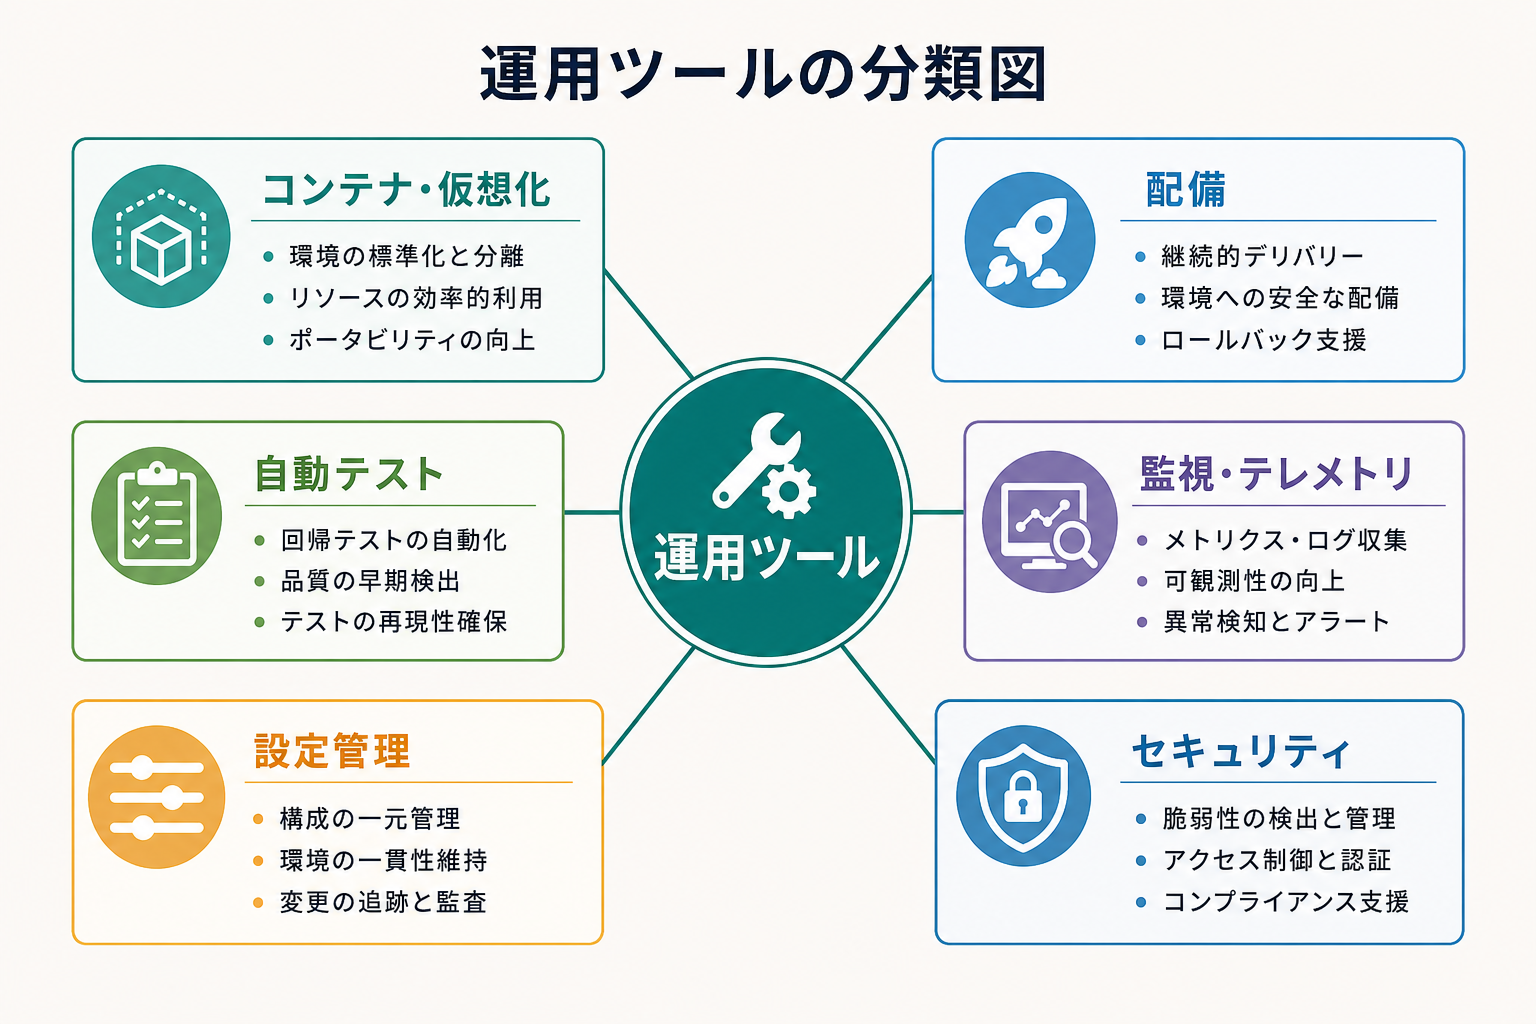
\includegraphics[width=0.96\linewidth]{assets/generated_figures/ch06/fig-ch06-12.png}}{\fbox{\parbox[c][48mm][c]{0.9\linewidth}{\centering 画像生成待ち\\運用ツールの分類図}}}
\caption{運用ツールの分類図}
\label{fig:ch06-12}
\end{figure}
